
\section{Numerical examples}\label{examples}
In this section, several examples are carried out to verify proposed method, which employs the consistent reproducing kernel gradient smoothing integration scheme (RKGSI) and the non-consistent Gauss integration scheme (GI) with penalty method, Nitsche's method and the proposed Hu-Washizu formulation (HW) to enforce the essential boundary conditions. A normalized support size of 2.5 is used for all methods to ensure the requirement of quadratic base meshfree approximation. To eliminate the influence of integration, the Gauss integration scheme use 6 Gauss points for domain integration and 3 points for boundary integration, and such that the number of integration points are identical between Gauss scheme and RKGSI scheme. The error estimates of displacement namely $L_2$-Error and energy namely $H_e$-Error is used here:
\begin{equation}
\begin{split}
L_2\text{-Error} &= \frac{\sqrt{\int_\Omega(\boldsymbol v - \boldsymbol v^h) \cdot (\boldsymbol v - \boldsymbol v^h)d\Omega}}{\sqrt{\boldsymbol v \cdot \boldsymbol v}} \\
H_e\text{-Error} &= \frac{\sqrt{\int_\Omega \left ((\varepsilon_{\alpha\beta} - \varepsilon_{\alpha\beta}^h)(N^{\alpha\beta} - N^{\alpha\beta h}) + \int_\Omega(\kappa_{\alpha\beta}-\kappa_{\alpha\beta}^h)(M^{\alpha\beta}-M^{\alpha\beta h}) \right )d\Omega}}{\sqrt{\int_\Omega(\varepsilon_{\alpha\beta}N^{\alpha\beta} + \kappa_{\alpha\beta}M^{\alpha\beta})d\Omega}}
\end{split}
\end{equation}

\subsection{Patch tests}
The linear and quadratic patch tests for flat and curved thin shell are firstly study to verify the variational consistency of the proposed method. As shown in Fig. \ref{ptf1}, the flat and curved model is depicted by an identical parametric domain $\Omega = (0,1)\otimes(0,1)$, where the cylindrical coordinate system with radius $R=1$ is employed to describe the curved model, and the whole domain $\Omega$ is discretized by $165$ meshfree nodes. All the boundaries are enforced as essential boundary conditions with the following manufactured exact solution:
\begin{equation}
\boldsymbol v = \begin{Bmatrix}
(\xi^1+2\xi^2)^n \\ (3\xi^1+4\xi^2)^n \\ (5\xi^1+6\xi^2)^n
\end{Bmatrix},\quad
n = \begin{cases}
1 & \text{Linear patch test} \\
2 & \text{Quadratic patch test}
\end{cases}
\end{equation}

\begin{figure}[h!]
    \centering
    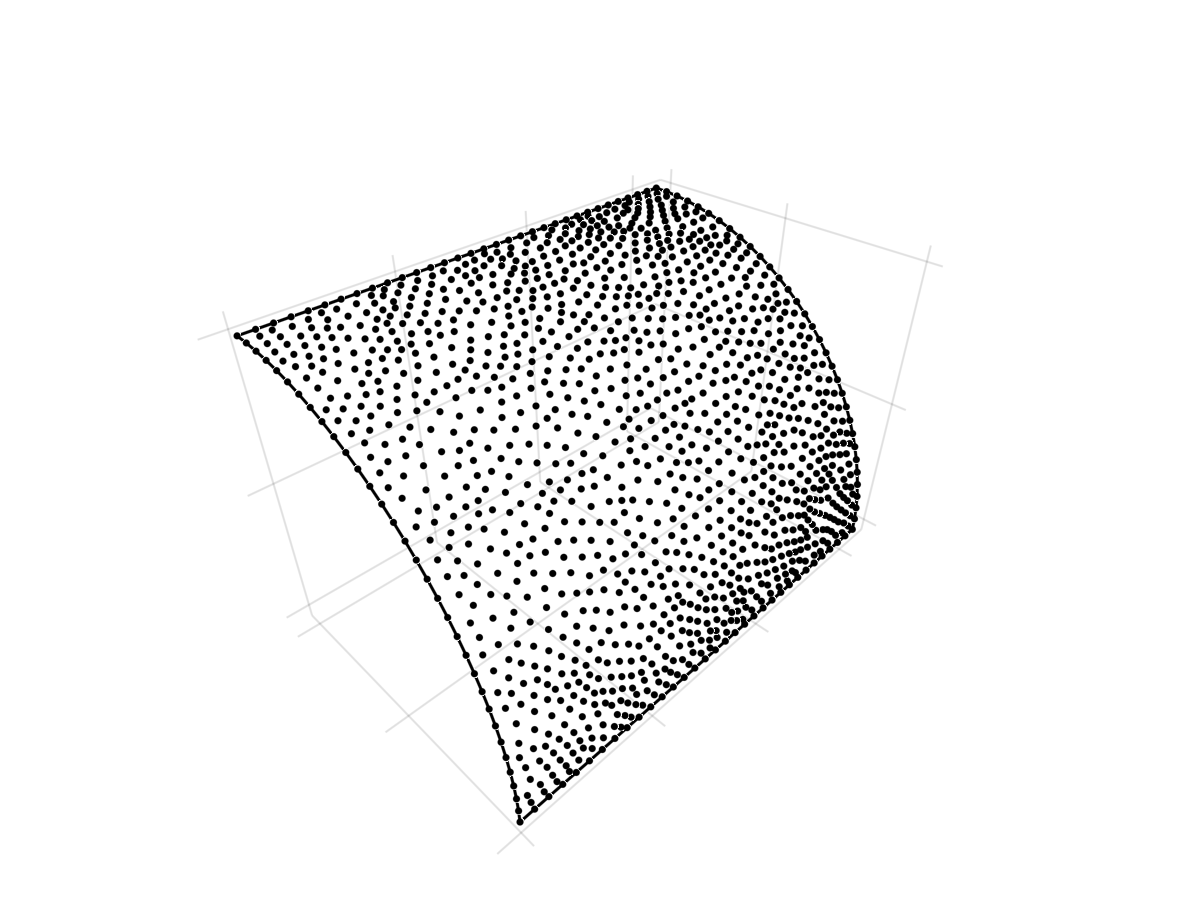
\includegraphics[width=\textwidth]{figures/patchtest_msh}
    \caption{Meshfree discretization for patch test}\label{ptf1}
\end{figure}

Table \ref{ptt1} lists the $L_2$- and $H_e$-Error results of patch test with flat model, where the RKGSI with variational consistent essential boundary enforcement, i.e. RKGSI-Nitsche and RKGSI-HW, can pass the linear and quadratic path test. Due to the loss of variational consistency condition, even with Nitsche's method, Gauss meshfree formulations show noticeable errors. Table \ref{ptt2} shows the results for curved model, which indicated that all the mehtods cannot pass the patch test, which mainly because the proposed smoothed gradient of Eqs. (\ref{approxse1}), (\ref{approxse2}) is unable to exactly reproduce the non-polynomial membrane and bending stress. However, the RKGSI-HW and RKGSI-Nitsche also performance better accuracy than other methods due to the fulfillment of first two order variational consistency. Meanwhile, the bending moment contours of $M^{12}$ are listed in Fig. \ref{ptf2}, which further verify that the proposed method obtain a satisfactory result comparing with exact solution, the conventional Gauss meshree formulations show observable errors.

\begin{table}[h!]
\centering
\caption{Results of patch test for flat model}\label{ptt1}
\begin{tabular}{lcccc}
\toprule
 & \multicolumn{2}{c}{Linear patch test} & \multicolumn{2}{c}{Quadratic patch test} \\ \cline{2-5}
 & $L_2$-Error & $H_e$-Error & $L_2$-Error & $H_e$-Error \\
    \midrule
    GI-Penalty & $4.45E-4$ & $1.35E-2$ & $2.01E-3$ & $1.63E-2$ \\
    GI-Nitsche & $4.51E-4$ & $1.42E-2$ & $1.22E-3$ & $1.68E-2$ \\
    RKGSI-Penalty & $3.64E-9$ & $6.77E-8$ & $4.54E-9$ & $6.57E-8$ \\
    RKGSI-Nitsche & $3.31E-12$ & $1.34E-11$ & $5.98E-12$ & $1.21E-11$ \\
    RKGSI-HR & $6.67E-13$ & $1.50E-11$ & $1.07E-12$ & $1.26E-11$ \\
    \bottomrule
\end{tabular}
\end{table}

\begin{table}[h!]
\centering
\caption{Results of patch test for curved model.}\label{ptt2}
\begin{tabular}{lcccc}
\toprule
 & \multicolumn{2}{c}{Linear patch test} & \multicolumn{2}{c}{Quadratic patch test} \\ \cline{2-5}
 & $L_2$-Error & $H_e$-Error & $L_2$-Error & $H_e$-Error \\
    \midrule
    GI-Penalty & $3.79E-4$ & $1.30E-2$ & $1.74E-3$ & $1.37E-2$ \\
    GI-Nitsche & $4.04E-4$ & $1.42E-2$ & $1.15E-3$ & $1.49E-2$ \\
    RKGSI-Penalty & $1.47E-4$ & $5.39E-3$ & $2.26E-4$ & $2.09E-3$ \\
    RKGSI-Nitsche & $2.41E-6$ & $7.37E-5$ & $2.47E-6$ & $2.89E-5$ \\
    RKGSI-HR & $4.28E-6$ & $1.30E-4$ & $9.69E-6$ & $2.41E-4$ \\
    \bottomrule
\end{tabular}
\end{table}

\begin{figure}[h!]
\centering
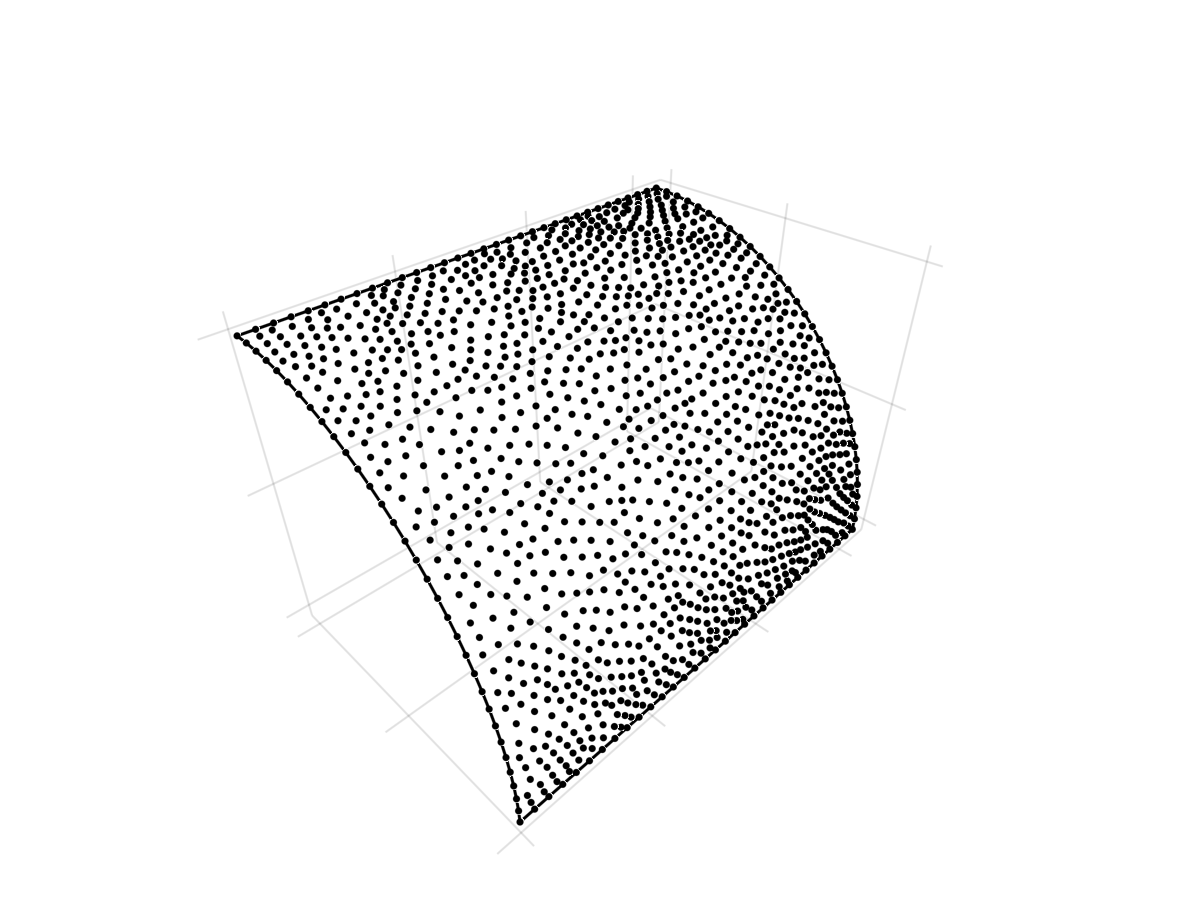
\includegraphics[width=\textwidth]{figures/patchtest_msh}
\caption{Contour plots of $M^{12}$ for curved shell patch test.}\label{ptf2}
\end{figure}

\subsection{Scordelis-Lo roof}
This example consider the classical Scordelis-Lo roof problem, as shown in Fig., the cylindrical roof has the radius $R=25$, length $L=50$, thickness $h=0.25$, Young's modulus $E=4.32\times 10^8$ and Poisson rate $\nu=0.0$. An uniform body force of $b_z = -90$ are enforced in whole roof and the curved edges are enforced by $v_x=v_z=0$, and the straight edges are free.

Due to the symmetry, only a quadrant of the model is considered for meshfree analysis, which is discretized by the $5\times 8$, $11\times 16$, $17\times 24$ and $23\times32$ meshfree nodes.

\begin{figure}[h!]
\centering
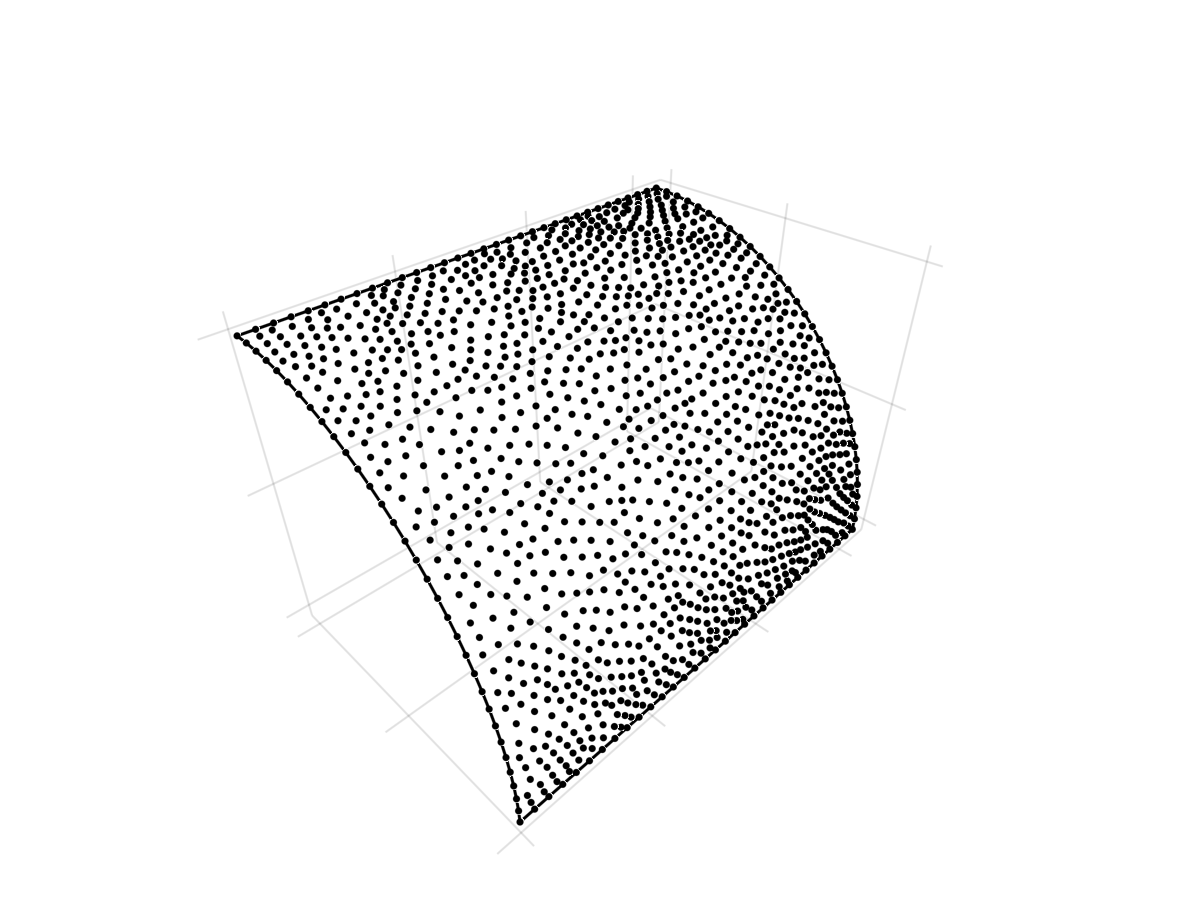
\includegraphics[width=\textwidth]{figures/patchtest_msh}
\caption{Description of Scordelis-Lo roof problem.}\label{ptf2}
\end{figure}
